\documentclass[a4paper]{article}
\usepackage{graphicx}
\usepackage{xcolor}
\usepackage{url}
\usepackage{outlines}
\usepackage{listings}
\usepackage{fontspec}
\lstset{basicstyle=\ttfamily,
	showstringspaces=false,
	commentstyle=\color{gray},
	keywordstyle=\color{pink}
}
\lstset{emph={
	nc,tcp,udp,http,openssl,sha256sum,},emphstyle=\color{purple}
}
\usepackage{fancyhdr}
\usepackage{geometry}
\geometry{
	a4paper,
	total={170mm,257mm},
	left=20mm,
	top=20mm,
	bottom=39mm,
}

\setlength{\headheight}{82.70538pt}

\fancypagestyle{oida}{
	\fancyhf{}
	\fancyhead[L]{\fontsize{7.5}{7.5}htl donaustadt\\ Donaustadtstraße 45\\
		1220 Wien\\~\\ Abteilung: Informationstechnologie\\ 
	Schwerpunkt: Netzwerktechnik}
	\fancyhead[R]{
\includegraphics[scale=0.45]{images/logo.png}}

	\fancyfoot[L]{\today}
	\fancyfoot[C]{\jobname}
	\fancyfoot[R]{Seite: \thepage}
}

\begin{document}
\bibliographystyle{plain}
\pagestyle{oida}
\section*{Kryptographie}
\par\noindent\rule{\textwidth}{0.4pt}

Laborprotokoll
Übung 3

\begin{figure}[h]
	
\includegraphics[scale=0.3]{images/mika.jpeg}
	\caption{Wunderbares Gruppenbild}
\end{figure}

\vspace*{\fill}
Unterrichtsgegenstand:	ITSI|ZIVK

Jahrgang:	3AHITN

Name:	Stefan Fürst, Marcel Raichle

Gruppenname/Nummer: Dumm und Dümmer/7

Betreuer: 	ZIVK

Übungsdaten:	4.10.2024, 11.10.2024

Abgabedatum:	7.6.2024


\newpage
\tableofcontents

\newpage

\section{Aufgabenstellung}

Zunächst geht es um die symmetrische Verschlüsselung, bei der eine Datei mit einem berechneten Passwort verschlüsselt und anschließend wieder entschlüsselt wird. Hierbei dient dasselbe Passwort sowohl zur Verschlüsselung als auch zur Entschlüsselung, um den Prozess zu überprüfen und zu verifizieren.
\\\\
Im zweiten Teil wird die asymmetrische Verschlüsselung behandelt. Dabei werden ein privater und ein öffentlicher Schlüssel generiert, und die Datei wird mithilfe des öffentlichen Schlüssels verschlüsselt. Dieser Ansatz simuliert ein typisches Verschlüsselungsverfahren, bei dem der private Schlüssel zur Entschlüsselung verwendet wird.
\\\\
Zum Abschluss erfolgt eine Integritätsprüfung mit Hilfe von Hashwerten. Dabei werden mehrere Textdateien mit vorgegebenen Hashwerten verglichen, um sicherzustellen, dass keine Datenveränderungen stattgefunden haben. Ziel ist es zudem, einen Hashwert zu identifizieren, der keiner der Textdateien zugeordnet werden kann.

\section{Zusammenfassung}


\newpage

\section{Übungsdurchführung}
\subsection{Symmetrisch Verschlüsseln}
\subsubsection{ Passwort für die Symetrische verschlüsselung berechnen}
$$\frac{Datum+Katalognummer}{2}$$
$$\frac{20241004+24}{2}$$
\subsubsection{Datei Symetrisch mit AES256 verschlüsseln}
Hierfür benutzt man openssl, ein kryptographisches Toolkit.\cite{openssl-cheatsh}\\
Um in diesem Fall die Datei mit AES256 zu verschlüsseln, man verwendet aes256 als Argument und die Flags \texttt{-in/out} geben die input/outputdatei an. Nach der Eingagbe des Commands, muss man ein Passwort eingeben.
\begin{figure}[h]
	\centering
	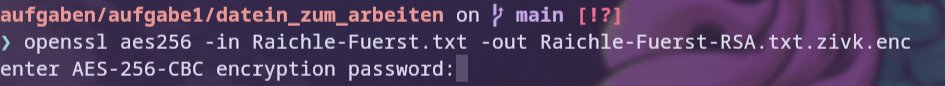
\includegraphics[scale=1.5]{images/aes-encrypt.png}
	\caption{AES entschlüsselung}
\end{figure} \\ \\
Für die Entschlüsselung wird die \texttt{-d} Flag verwendet, welche für decrypt steht, dies und das Austauschen von input und ouput werden benötigt, um die Datei zu entschlüsseln. Wenn der Command ausgeführt wurde, wird das Passwort abgefragt.
\begin{figure}[h]
	\centering
	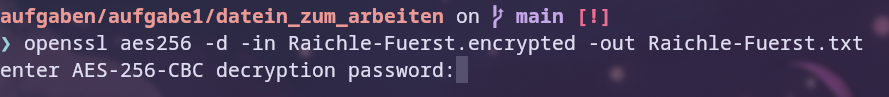
\includegraphics[scale=1.5]{images/aes-decrypt.png}
	\caption{AES entschlüsselung}
\end{figure}
\begin{lstlisting}[language=bash]
#verschlüsseln
openssl aes256 -in Raichle.txt -out Raichle.encrypted
#entschlüsseln
openssl aes256 -d -in Raichle.encrypted -out Raichle.txt
\end{lstlisting}

\subsection{Asymmetrisch Verschlüsseln}
Für die Asymetrische Verschlüsselung, müssen erst ein Keypair generiert werden.
%größe andern dass alles drauf is
\begin{lstlisting}[language=bash]
#public key
openssl genpkey -algorithm RSA -pkeyopt rsa_keygen_bits:4096 -out private-key.pem
#private key
openssl pkey -in private-key.pem -out public-key.pem -pubout
#datei verschlüsseln
openssl rsautl -encrypt -inkey zivk.pem -pubin -in Raichle-Fuerst-RSA.txt -out Raichle-Fuerst-RSA.txt.zivk.enc
\end{lstlisting}

\subsection{Integrität prüfen}
\begin{lstlisting}[language=bash]
#benötigter command
sha256sum <dateiname>
\end{lstlisting}

\begin{figure}[h]
	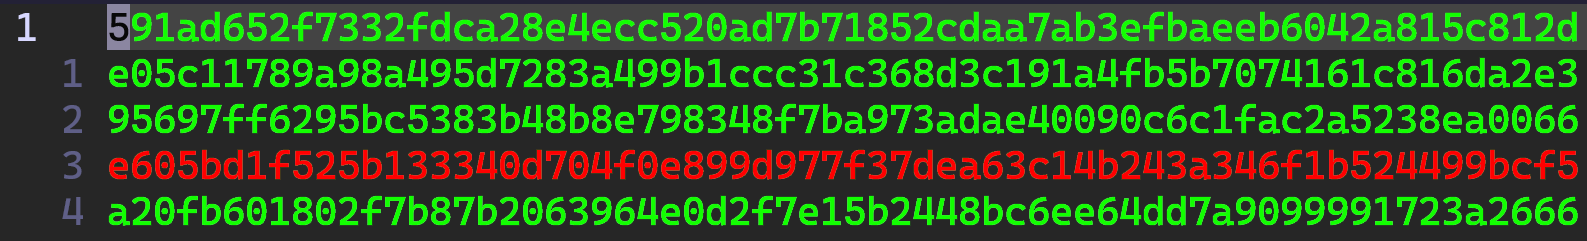
\includegraphics[scale=0.3]{images/hashes.png}
	\caption{Hashes}
\end{figure}

% der 3te hat keinen hash


\newpage
\section{Quellen}
\bibliography{quellen}
\newpage
\section{Abbildungsverzeichnis}

\listoffigures

\end{document}
